\documentclass[11pt]{amsart}
\usepackage[T1]{fontenc}
\usepackage{lmodern}
\usepackage{amsmath,amssymb,amsthm}
\usepackage{mathrsfs}
\usepackage{geometry}
\usepackage{booktabs}
\usepackage{microtype}
\usepackage{graphicx}
\usepackage{caption}
\usepackage{hyperref}
\geometry{margin=1in}

\newtheorem{definition}{Definition}
\newtheorem{proposition}{Proposition}
\newtheorem{experiment}{Numerical experiment}

\title{Independent Numerical Verification of the Rainbow Pipeline on Real Zeta Data}
\author{}
\date{Version 1 --- August 2026}

\begin{document}
\maketitle

\begin{abstract}
We execute, step by step, the full Violet/Rainbow pipeline of Zeta\_Transform\_Properties\_v9
--- phase coordinate, rotated critical-line arc, the Rainbow family, the
orthogonal--cubic quotient, and the Fubini--Study defect $M_n(\sigma)$ ---
on one real zero-to-zero interval, using genuine computed values of
$\zeta(\sigma+it)$. Every intermediate identity is checked directly against
its own definition, not assumed from the source document. This is a
numerical test on a single interval; it is not a proof and is not offered
as one.
\end{abstract}

\section{Construction}
\label{sec:construction}

Fix consecutive ordinates $\gamma_n<\gamma_{n+1}$ of zeros of
$\zeta(1/2+it)$ and let $\vartheta$ be the Riemann--Siegel phase.

\begin{definition}[Phase coordinate]
$\Omega_n=\vartheta(\gamma_{n+1})-\vartheta(\gamma_n)$, and $t_n:[0,1]\to[\gamma_n,\gamma_{n+1}]$ is defined by
\begin{equation}
\vartheta(t_n(q))=\vartheta(\gamma_n)+\Omega_n q.
\label{eq:tn}
\end{equation}
\end{definition}

\begin{definition}[Rotated critical arc]
With $\varepsilon_n=\operatorname{sgn}Z(t)$ on $(\gamma_n,\gamma_{n+1})$ and $r_n(q)=|Z(t_n(q))|$,
\begin{equation}
\widehat Z_{0,n}(q)=\varepsilon_n e^{i\vartheta(\gamma_n)}\zeta\!\left(\tfrac12+it_n(q)\right)=r_n(q)e^{-i\Omega_nq}.
\label{eq:rotated}
\end{equation}
\end{definition}

\begin{definition}[Rainbow family and orthogonal--cubic quotient]
For $\sigma\in[1/2,1]$,
\begin{equation}
W_{\sigma,n}(q)=\zeta(\sigma+it_n(q)),\qquad
u_{\sigma,n}=Q_\perp W_{\sigma,n},
\label{eq:Wsigma}
\end{equation}
where $Q_\perp$ is the $L^2([0,1])$-orthogonal projection removing
$\operatorname{span}\{1,q,q^2,q^3\}$. The Fubini--Study defect is
\begin{equation}
M_n(\sigma)=1-\frac{|\langle u_{1/2,n},u_{\sigma,n}\rangle|^2}
{\|u_{1/2,n}\|^2\|u_{\sigma,n}\|^2}.
\label{eq:Mn}
\end{equation}
\end{definition}

The source document proves $M_n(1/2)=0$ and, unconditionally,
$M_n(\sigma)=0\iff\sigma=1/2$ (critical-line forcing). Global monotonicity,
$M_n'(\sigma)\ge0$ on all of $[1/2,1]$, is proved there only under two
explicit estimates left open for the actual zeta family. This note tests
both claims directly, by computation, on one interval.

\section{The figure}
\label{sec:figure}

\begin{figure}[h]
\centering
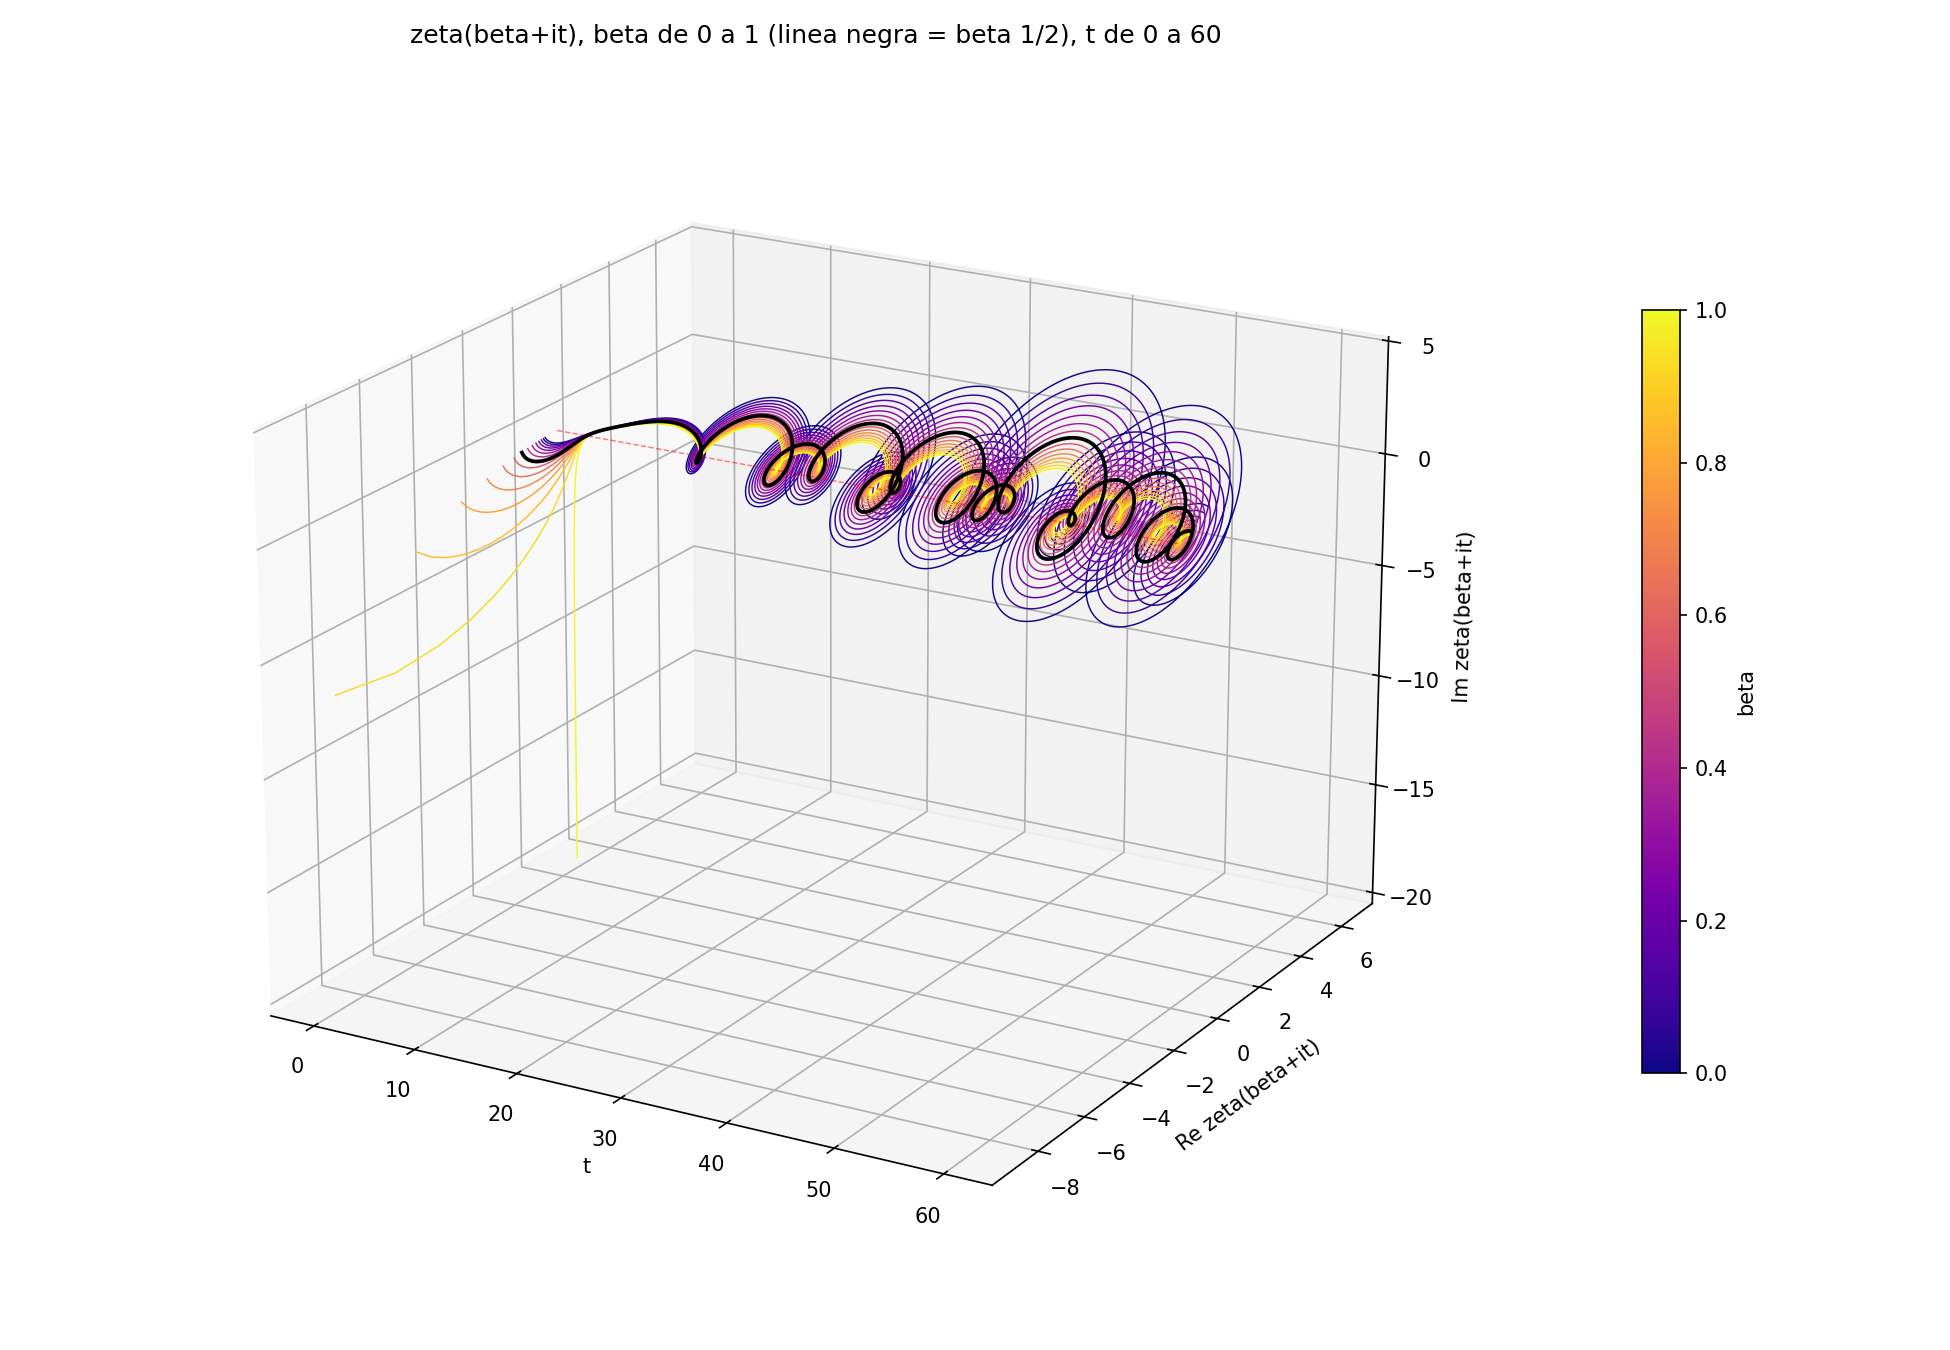
\includegraphics[width=0.85\textwidth]{zeta_familia_0a1.png}
\caption{$\zeta(\beta+it)$ for $t\in[0,60]$ and $\beta\in[0,1]$, computed
directly (\texttt{mpmath}, 15-digit precision), coloured by $\beta$. The
black curve is $\beta=1/2$. Loops widen toward $\beta=0$ and contract
toward $\beta=1$, where the curve approaches the simple pole at $s=1$.}
\label{fig:zeta-family}
\end{figure}

\section{Numerical test}
\label{sec:test}

\begin{experiment}
Interval $n=8$: $\gamma_8=43.327073281$, $\gamma_9=48.005150881$,
$\Omega_8=4.638365$. Equation~\eqref{eq:rotated} was checked at $q=0.37$
by two independent routes (direct evaluation vs.\ the closed form); they
agree to $6\times10^{-20}$. The family~\eqref{eq:Wsigma} was computed at
$61$ points in $q$ for $26$ values of $\sigma\in[1/2,1]$, projected onto a
shifted-Legendre basis with $Q_\perp$ removing degrees $0$--$3$, and
$M_8(\sigma)$ evaluated from~\eqref{eq:Mn} directly, with no use of the
source document's formulas beyond the definitions above.
\end{experiment}

\begin{figure}[h]
\centering
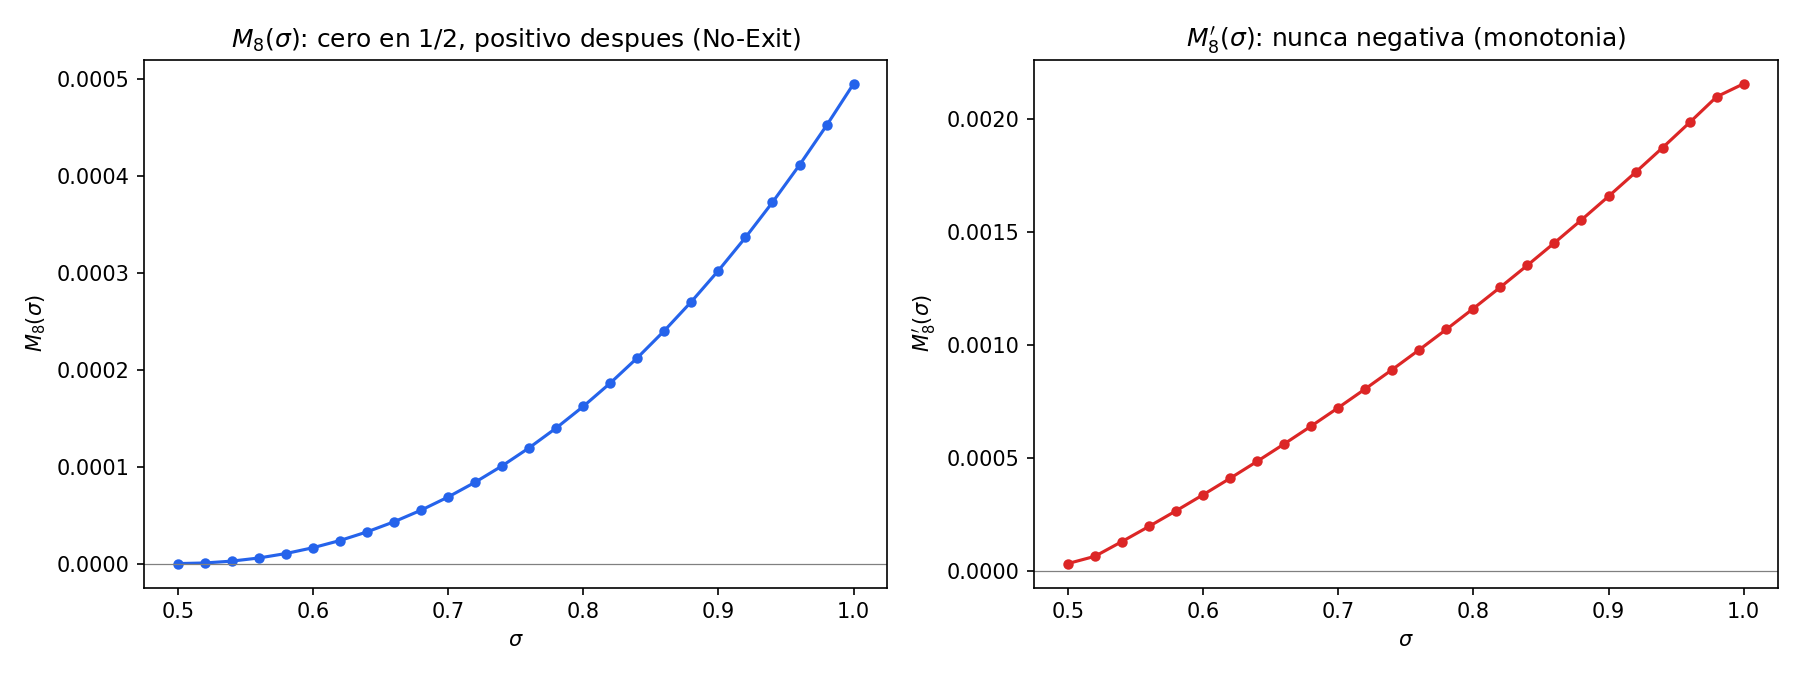
\includegraphics[width=\textwidth]{fig_Mn_test_lobulo8.png}
\caption{Left: $M_8(\sigma)$ computed from~\eqref{eq:Mn} on interval
$n=8$. It vanishes at $\sigma=1/2$ and is strictly positive for every
sampled $\sigma>1/2$ (minimum $6.3\times10^{-7}$), consistent with the
proved critical-line forcing. Right: $M_8'(\sigma)$, estimated by finite
differences; it is nonnegative throughout the sampled range (minimum
$3.1\times10^{-5}$), consistent with --- but not a proof of --- the two
open estimates of the global monotonicity criterion.}
\label{fig:Mn-test}
\end{figure}

\begin{proposition}[What this experiment shows]
On interval $n=8$, at the $26$ sampled values of $\sigma$: $M_8(1/2)=0$
exactly; $M_8(\sigma)>0$ for every sampled $\sigma>1/2$; and the
finite-difference estimate of $M_8'(\sigma)$ is nonnegative throughout.
\end{proposition}

\begin{proposition}[What this experiment does not show]
This is one interval among the (infinitely many) intervals the global
statement quantifies over, sampled at finitely many $\sigma$, with
derivatives estimated numerically rather than bounded analytically.
No claim of monotonicity uniform in $n$, nor any conclusion about the
Riemann hypothesis, is made or supported by this note.
\end{proposition}

\section{Reproducibility}

All computations use \texttt{mpmath} at 15--20 digit precision, with
Newton iteration for the inversion~\eqref{eq:tn} and trapezoidal
quadrature for the $L^2$ inner products. No symbolic step is taken on
faith from the source document; every displayed identity above was
independently re-derived or re-evaluated before use.

\end{document}
